\documentclass[tikz,border=5]{standalone}

% Drawing
\usepackage{tikz}

% Tikz Library
\usetikzlibrary{angles, quotes, decorations.markings}

%Styles

%%Arrow in the Middle
\tikzset{midarrow1/.style = {postaction=decorate, decoration={markings,mark=at position .8 with \arrow{stealth}}}}
\tikzset{midarrow2/.style = {postaction=decorate, decoration={markings,mark=at position .4 with \arrow{stealth}}}}
\tikzset{midarrow/.style={midarrow1, midarrow2}}


% Define Color
\definecolor{lust}{rgb}{0.9, 0.13, 0.13}
\definecolor{richelectricblue}{rgb}{0.03, 0.57, 0.82}

\begin{document}
	
	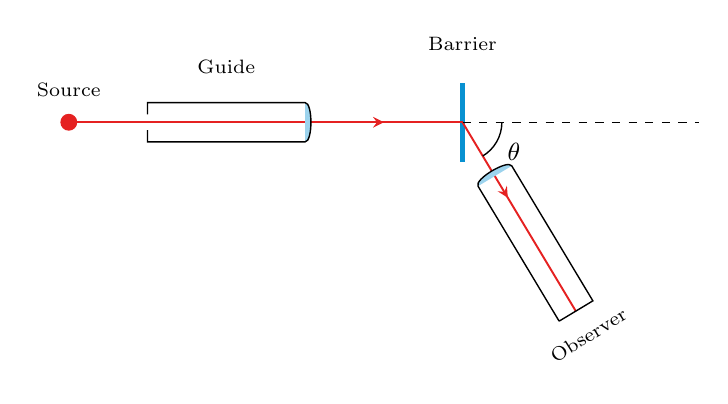
\begin{tikzpicture}
		
		% Barrier
		\draw[line width = 2, color = richelectricblue] (4,7.5) -- ++(0,1);
		
		% Rays
		\draw[color = lust, line width = 0.7, midarrow1] (-1,8) -- (4,8);
		\draw[color = lust, line width = 0.7, midarrow2] (4,8) -- +(3*24/50,-5*24/50) coordinate (C);
		
		% Guide and Lens
		%% Top
		\path[fill = richelectricblue!40] (2,8.25) ..controls +(0.1,0) and +(0.1,0).. ++(0,-0.5) ;
		\draw[line width = 0.5] (0, 8.1) -- (0,8.25) -- ++(2,0) ..controls +(0.1,0) and +(0.1,0).. ++(0,-0.5) -- ++(-2,0) -- +(0, 0.15);
		%% Bottom
		\path[fill = richelectricblue!40, rotate = 121] (4,-7.3) ..controls +(0.1,0) and +(0.1,0).. ++(0,-0.5) ;
		\draw[line width = 0.5, rotate = 121] (2,-7.3) -- ++(2,0) ..controls +(0.1,0) and +(0.1,0).. ++(0,-0.5) -- ++(-2,0) -- +(0,0.50);
		
		% Source		
		\draw [fill = lust, draw = lust] (-1,8) circle [radius=0.1];
		
		% Dashed
		\draw[dashed, line width = 0.5] (4,8)coordinate(A) -- ++(3,0)coordinate(B);
		
		% Angle
		\pic[draw , "\small$\theta$", line width = 0.5, angle radius=0.5cm, angle eccentricity = 1.5] {angle=C--A--B};
		
		% Nodes
		\node[above] at (-1,8.2) {\scriptsize Source};
		\node[above] at (1,8.5) {\scriptsize Guide};
		\node at (4,9) {\scriptsize Barrier};
		\node[rotate=32] at (5.6,5.3) {\scriptsize Observer}; 
	\end{tikzpicture}
	
\end{document}